\chapter{Consultes d'interval}

\index{consulta d'interval} \index{consulta de suma} \index{consulta de mínim}
\index{consulta de màxim}

En aquest capítol parlem de les estructures de dades que ens permeten
processar de manera eficient les consultes d'interval. En una
\key{consulta d'interval}, la nostra tasca és calcular un valor basat
en un subvector d'un vector. Les consultes d'interval típiques són:
\begin{itemize}
\item $\texttt{sum}_q(a,b)$: calculate the sum of values in range $[a,b]$
\item $\texttt{min}_q(a,b)$: find the minimum value in range $[a,b]$
\item $\texttt{max}_q(a,b)$: find the maximum value in range $[a,b]$
\end{itemize}


Per exemple, considereu l'interval $[3,6]$ al vector següent:
\begin{center}
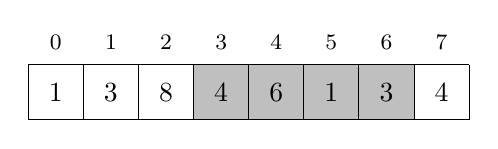
\begin{tikzpicture}[scale=0.7]
\fill[color=lightgray] (3,0) rectangle (7,1);
\draw (0,0) grid (8,1);

\node at (0.5,0.5) {$1$};
\node at (1.5,0.5) {$3$};
\node at (2.5,0.5) {$8$};
\node at (3.5,0.5) {$4$};
\node at (4.5,0.5) {$6$};
\node at (5.5,0.5) {$1$};
\node at (6.5,0.5) {$3$};
\node at (7.5,0.5) {$4$};

\footnotesize
\node at (0.5,1.4) {$0$};
\node at (1.5,1.4) {$1$};
\node at (2.5,1.4) {$2$};
\node at (3.5,1.4) {$3$};
\node at (4.5,1.4) {$4$};
\node at (5.5,1.4) {$5$};
\node at (6.5,1.4) {$6$};
\node at (7.5,1.4) {$7$};
\end{tikzpicture}
\end{center}
En aquest cas, $\texttt{sum}_q(3,6)=14$, $\texttt{min}_q(3,6)=1$ i
$\texttt{max}_q(3,6)=6 $.

Una manera senzilla de processar les consultes d'interval és fer
servir un bucle que recorre tots els valors de matriu de
l'interval. Per exemple, la funció següent es pot fer servir per
processar consultes de suma en un vector:


\begin{lstlisting}
int sum(int a, int b) {
    int s = 0;
    for (int i = a; i <= b; i++) {
        s += array[i];
    }
    return s;
}
\end{lstlisting}


Aquesta funció funciona en temps $O(n)$, on $n$ és la mida del
vector. Així, podem processar $q$ consultes en temps $O(nq)$
fent servir la funció. Tanmateix, si $n$ i $q$ són grans, aquest
enfocament és lent. Afortunadament, resulta que hi ha maneres de
processar les consultes d'interval de manera molt més eficient.

\section{Consultes de vector estàtiques}

Primer ens centrem en una situació en què el vector és \emph{estàtic},
és a dir, els valors del vector mai canvien entre consultes. En aquest
cas, n'hi ha prou amb construir una estructura de dades estàtica que
ens indiqui la resposta a qualsevol consulta possible.

\subsubsection{Consultes de suma}

\index{vector suma de prefixos}

Podem processar fàcilment les consultes de suma en un vector estàtic
mitjançant la construcció d'un vector suma de prefixos (\key{prefix
  sum array}). Cada valor del vector suma de prefixos és igual a la
suma de valors del vector original fins a aquesta posició, és a dir,
el valor a la posició $k$ és $\texttt{sum}_q(0,k)$. El vector suma de
prefixos es pot construir en temps $O(n)$.

Per exemple, considereu el vector següent:
\begin{center}
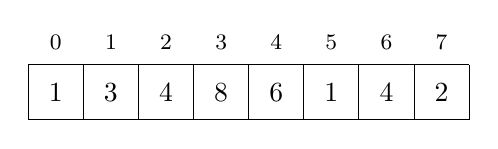
\begin{tikzpicture}[scale=0.7]
%\fill[color=lightgray] (3,0) rectangle (7,1);
\draw (0,0) grid (8,1);

\node at (0.5,0.5) {$1$};
\node at (1.5,0.5) {$3$};
\node at (2.5,0.5) {$4$};
\node at (3.5,0.5) {$8$};
\node at (4.5,0.5) {$6$};
\node at (5.5,0.5) {$1$};
\node at (6.5,0.5) {$4$};
\node at (7.5,0.5) {$2$};

\footnotesize
\node at (0.5,1.4) {$0$};
\node at (1.5,1.4) {$1$};
\node at (2.5,1.4) {$2$};
\node at (3.5,1.4) {$3$};
\node at (4.5,1.4) {$4$};
\node at (5.5,1.4) {$5$};
\node at (6.5,1.4) {$6$};
\node at (7.5,1.4) {$7$};
\end{tikzpicture}
\end{center}
El vector suma de prefixos corresponent és:
\begin{center}
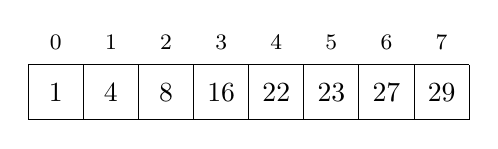
\begin{tikzpicture}[scale=0.7]
%\fill[color=lightgray] (3,0) rectangle (7,1);
\draw (0,0) grid (8,1);

\node at (0.5,0.5) {$1$};
\node at (1.5,0.5) {$4$};
\node at (2.5,0.5) {$8$};
\node at (3.5,0.5) {$16$};
\node at (4.5,0.5) {$22$};
\node at (5.5,0.5) {$23$};
\node at (6.5,0.5) {$27$};
\node at (7.5,0.5) {$29$};


\footnotesize
\node at (0.5,1.4) {$0$};
\node at (1.5,1.4) {$1$};
\node at (2.5,1.4) {$2$};
\node at (3.5,1.4) {$3$};
\node at (4.5,1.4) {$4$};
\node at (5.5,1.4) {$5$};
\node at (6.5,1.4) {$6$};
\node at (7.5,1.4) {$7$};
\end{tikzpicture}
\end{center}
Com que el vector suma de prefixos conté tots els valors de
$\texttt{sum}_q(0,k)$, podem calcular qualsevol valor de
$\texttt{sum}_q(a,b)$ en temps $O(1)$ com segueix:
\[ \texttt{sum}_q(a,b) = \texttt{sum}_q(0,b) - \texttt{sum}_q(0,a-1)\]
Definit $\texttt{sum}_q(0,-1)=0$, la fórmula anterior també es compleix quan $a=0$.

Per exemple, considereu l'interval $[3,6]$:
\begin{center}
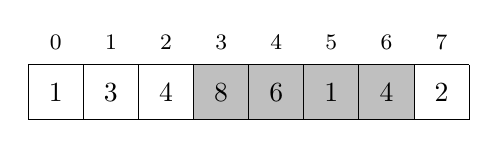
\begin{tikzpicture}[scale=0.7]
\fill[color=lightgray] (3,0) rectangle (7,1);
\draw (0,0) grid (8,1);

\node at (0.5,0.5) {$1$};
\node at (1.5,0.5) {$3$};
\node at (2.5,0.5) {$4$};
\node at (3.5,0.5) {$8$};
\node at (4.5,0.5) {$6$};
\node at (5.5,0.5) {$1$};
\node at (6.5,0.5) {$4$};
\node at (7.5,0.5) {$2$};

\footnotesize
\node at (0.5,1.4) {$0$};
\node at (1.5,1.4) {$1$};
\node at (2.5,1.4) {$2$};
\node at (3.5,1.4) {$3$};
\node at (4.5,1.4) {$4$};
\node at (5.5,1.4) {$5$};
\node at (6.5,1.4) {$6$};
\node at (7.5,1.4) {$7$};
\end{tikzpicture}
\end{center}
En aquest cas $\texttt{sum}_q(3,6)=8+6+1+4=19$. Aquesta suma es pot
calcular a partir de dos valors de la matriu de suma de prefix:
\begin{center}
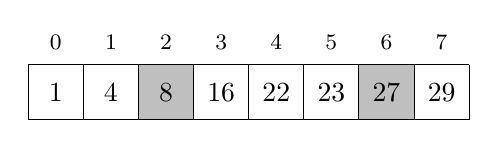
\begin{tikzpicture}[scale=0.7]
\fill[color=lightgray] (2,0) rectangle (3,1);
\fill[color=lightgray] (6,0) rectangle (7,1);
\draw (0,0) grid (8,1);

\node at (0.5,0.5) {$1$};
\node at (1.5,0.5) {$4$};
\node at (2.5,0.5) {$8$};
\node at (3.5,0.5) {$16$};
\node at (4.5,0.5) {$22$};
\node at (5.5,0.5) {$23$};
\node at (6.5,0.5) {$27$};
\node at (7.5,0.5) {$29$};

\footnotesize
\node at (0.5,1.4) {$0$};
\node at (1.5,1.4) {$1$};
\node at (2.5,1.4) {$2$};
\node at (3.5,1.4) {$3$};
\node at (4.5,1.4) {$4$};
\node at (5.5,1.4) {$5$};
\node at (6.5,1.4) {$6$};
\node at (7.5,1.4) {$7$};
\end{tikzpicture}
\end{center}
Així, $\texttt{sum}_q(3,6)=\texttt{sum}_q(0,6)-\texttt{sum}_q(0,2)=27-8=19$.

També és possible generalitzar aquesta idea a dimensions
superiors. Per exemple, podem construir una matriu de suma de prefixos
bidimensional que es pot utilitzar per calcular la suma de qualsevol
submatriu rectangular en temps $O(1)$. Cada suma d'aquesta matriu
correspon a una submatriu que comença a la cantonada superior esquerra
de la matriu.


\begin{samepage}
The following picture illustrates the idea:
\begin{center}
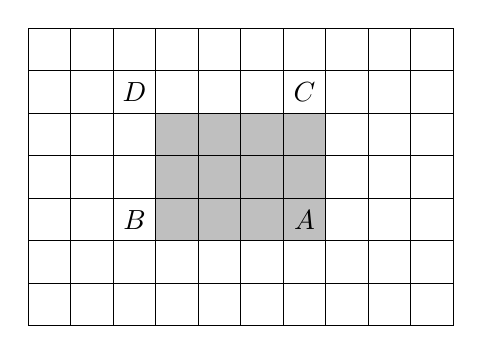
\begin{tikzpicture}[scale=0.54]
\draw[fill=lightgray] (3,2) rectangle (7,5);
\draw (0,0) grid (10,7);
\node[anchor=center] at (6.5, 2.5) {$A$};
\node[anchor=center] at (2.5, 2.5) {$B$};
\node[anchor=center] at (6.5, 5.5) {$C$};
\node[anchor=center] at (2.5, 5.5) {$D$};
\end{tikzpicture}
\end{center}
\end{samepage}


La suma de la submatriu gris es pot calcular mitjançant la fórmula
\[S(A) - S(B) - S(C) + S(D),\]
on $S(X)$ indica la suma de valors d'una submatriu des de la cantonada superior
esquerra fins a la posició de $X$.

\subsubsection{Consultes mínimes}

\index{vector dispers}

Les consultes de mínim són més difícils de resoldre que les consultes
de suma. Tot i així, hi ha un mètode de preprocessament de temps $O(n
\log n)$ força senzill després del qual podem respondre qualsevol
consulta mínima en $temps O(1)$\footnote{Aquesta tècnica es va
introduir a \cite{ben00} i de vegades s'anomena mètode del vector dispersa
(\key{sparse array}). També hi ha tècniques més sofisticades \cite{fis06} on el
temps de preprocessament és només $O(n)$, però aquests algorismes no
són necessaris en la programació competitiva.}. Tingueu en compte que
com que les consultes mínimes i màximes es poden processar de manera
similar, ens podem centrar en les consultes mínimes.

La idea és precalcular tots els valors de $\textrm{min}_q(a,b)$ on
$b-a+1$ (la longitud de l'interval) és una potència de dos. Per
exemple, per al vector


\begin{center}
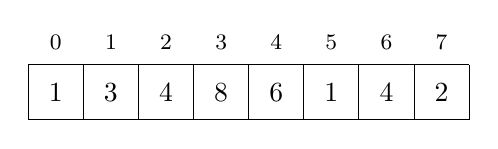
\begin{tikzpicture}[scale=0.7]
\draw (0,0) grid (8,1);

\node at (0.5,0.5) {$1$};
\node at (1.5,0.5) {$3$};
\node at (2.5,0.5) {$4$};
\node at (3.5,0.5) {$8$};
\node at (4.5,0.5) {$6$};
\node at (5.5,0.5) {$1$};
\node at (6.5,0.5) {$4$};
\node at (7.5,0.5) {$2$};

\footnotesize
\node at (0.5,1.4) {$0$};
\node at (1.5,1.4) {$1$};
\node at (2.5,1.4) {$2$};
\node at (3.5,1.4) {$3$};
\node at (4.5,1.4) {$4$};
\node at (5.5,1.4) {$5$};
\node at (6.5,1.4) {$6$};
\node at (7.5,1.4) {$7$};
\end{tikzpicture}
\end{center}
es calculen els valors següents:


\begin{center}
\begin{tabular}{ccc}

\begin{tabular}{lll}
$a$ & $b$ & $\texttt{min}_q(a,b)$ \\
\hline
0 & 0 & 1 \\
1 & 1 & 3 \\
2 & 2 & 4 \\
3 & 3 & 8 \\
4 & 4 & 6 \\
5 & 5 & 1 \\
6 & 6 & 4 \\
7 & 7 & 2 \\
\end{tabular}

&

\begin{tabular}{lll}
$a$ & $b$ & $\texttt{min}_q(a,b)$ \\
\hline
0 & 1 & 1 \\
1 & 2 & 3 \\
2 & 3 & 4 \\
3 & 4 & 6 \\
4 & 5 & 1 \\
5 & 6 & 1 \\
6 & 7 & 2 \\
\\
\end{tabular}

&

\begin{tabular}{lll}
$a$ & $b$ & $\texttt{min}_q(a,b)$ \\
\hline
0 & 3 & 1 \\
1 & 4 & 3 \\
2 & 5 & 1 \\
3 & 6 & 1 \\
4 & 7 & 1 \\
0 & 7 & 1 \\
\\
\\
\end{tabular}

\end{tabular}
\end{center}


El nombre de valors precalculats és $O(n \log n)$, perquè hi ha
$O(\log n)$ longituds d'interval que són potències de dos. Els valors
es poden calcular de manera eficient mitjançant la fórmula recursiva
\[\texttt{min}_q(a,b) = \min(\texttt{min}_q(a,a+w-1),\texttt{min}_q(a+w,b)),\]
on $b-a+1$ és una potència de dos i $w=(b-a+1)/2$. Calcular tots aquests valors
requereix temps $O(n \log n)$.

Després d'això, qualsevol valor de $\texttt{min}_q(a,b)$ es pot
calcular en temps $O(1)$ com el mínim de dos valors
precalculats. Sigui $k$ la potència de dos més gran que no superi
$b-a+1$. Podem calcular el valor de $\texttt{min}_q(a,b)$ mitjançant
la fórmula
\[\texttt{min}_q(a,b) = \min(\texttt{min}_q(a,a+k-1),\texttt{min}_q(b-k+1,b)).\]
A la fórmula anterior, l'interval $[a,b]$ es representa com la unió dels
intervals $[a,a+k-1]$ i $[b-k+1,b]$, tots dos de longitud $k$.

Com a exemple, considereu l'interval $[1,6]$:
\begin{center}
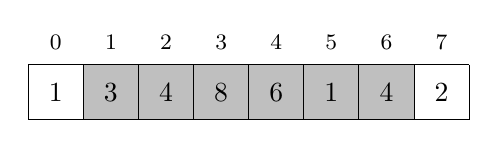
\begin{tikzpicture}[scale=0.7]
\fill[color=lightgray] (1,0) rectangle (7,1);
\draw (0,0) grid (8,1);

\node at (0.5,0.5) {$1$};
\node at (1.5,0.5) {$3$};
\node at (2.5,0.5) {$4$};
\node at (3.5,0.5) {$8$};
\node at (4.5,0.5) {$6$};
\node at (5.5,0.5) {$1$};
\node at (6.5,0.5) {$4$};
\node at (7.5,0.5) {$2$};

\footnotesize
\node at (0.5,1.4) {$0$};
\node at (1.5,1.4) {$1$};
\node at (2.5,1.4) {$2$};
\node at (3.5,1.4) {$3$};
\node at (4.5,1.4) {$4$};
\node at (5.5,1.4) {$5$};
\node at (6.5,1.4) {$6$};
\node at (7.5,1.4) {$7$};
\end{tikzpicture}
\end{center}
La longitud de l'interval és 6, i la potència més gran de dos que no supera 6 és 4. Així, el rang $[1,6]$ és la unió dels intervals $[1,4]$ i $[3, 6]$:
\begin{center}
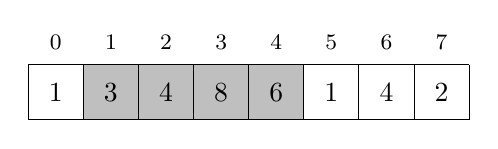
\begin{tikzpicture}[scale=0.7]
\fill[color=lightgray] (1,0) rectangle (5,1);
\draw (0,0) grid (8,1);

\node at (0.5,0.5) {$1$};
\node at (1.5,0.5) {$3$};
\node at (2.5,0.5) {$4$};
\node at (3.5,0.5) {$8$};
\node at (4.5,0.5) {$6$};
\node at (5.5,0.5) {$1$};
\node at (6.5,0.5) {$4$};
\node at (7.5,0.5) {$2$};

\footnotesize
\node at (0.5,1.4) {$0$};
\node at (1.5,1.4) {$1$};
\node at (2.5,1.4) {$2$};
\node at (3.5,1.4) {$3$};
\node at (4.5,1.4) {$4$};
\node at (5.5,1.4) {$5$};
\node at (6.5,1.4) {$6$};
\node at (7.5,1.4) {$7$};
\end{tikzpicture}
\end{center}

\begin{center}
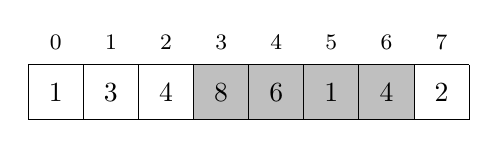
\begin{tikzpicture}[scale=0.7]
\fill[color=lightgray] (3,0) rectangle (7,1);
\draw (0,0) grid (8,1);

\node at (0.5,0.5) {$1$};
\node at (1.5,0.5) {$3$};
\node at (2.5,0.5) {$4$};
\node at (3.5,0.5) {$8$};
\node at (4.5,0.5) {$6$};
\node at (5.5,0.5) {$1$};
\node at (6.5,0.5) {$4$};
\node at (7.5,0.5) {$2$};


\footnotesize
\node at (0.5,1.4) {$0$};
\node at (1.5,1.4) {$1$};
\node at (2.5,1.4) {$2$};
\node at (3.5,1.4) {$3$};
\node at (4.5,1.4) {$4$};
\node at (5.5,1.4) {$5$};
\node at (6.5,1.4) {$6$};
\node at (7.5,1.4) {$7$};
\end{tikzpicture}
\end{center}
Com que $\texttt{min}_q(1,4)=3$ i $\texttt{min}_q(3,6)=1$, concloem
que $\texttt{min}_q(1,6)=1 $.

\section{Arbre binari indexat}

\index{arbre binari indexat} \index{arbre de Fenwick}

Un \key{arbre binari indexat} o un \key{arbre de
  Fenwick}\footnote{L'estructura d'arbre binari indexat va ser
presentada per P.M. Fenwick el 1994 \cite{fen94}.} es pot veure com una
variant dinàmica d'un vector suma de prefixos. Aquest admet dues
operacions de temps $O(\log n)$: processar una consulta de suma d'intervals i
actualitzar un valor.

L'avantatge d'un arbre binari indexat és que ens permet actualitzar de
manera eficient els valors del vector entre les consultes de
suma. Això no seria possible si fessim servir un vector suma de prefix,
perquè després de cada actualització, caldria tornar a reconstruir tot
el vector suma de prefix en temps $O(n)$.

\subsubsection{Estructura}

Encara que el nom de l'estructura sigui \emph{arbre} binari indexat,
normalment es representa com un vector. En aquesta secció suposem que
tots els vectors comencen amb index 1 (en lloc de 0), perquè dóna lloc
a una implementació més senzilla.

Sigui $p(k)$ la potència de dos més gran que divideix $k$. Emmagatzemem un arbre
binari indexat com un vector \texttt{arbre} de manera que
\[ \texttt{tree}[k] = \texttt{sum}_q(k-p(k)+1,k),\]
és a dir, cada posició $k$ conté la suma de valors en un interval del vector
original la longitud del qual és $p(k)$ i que acaba a la posició $k$. Per exemple, com que $p(6)=2$, $\texttt{tree}[6]$ conté el valor de $\texttt{sum}_q(5,6)$.

Per exemple, considereu el vector següent:
\begin{center}
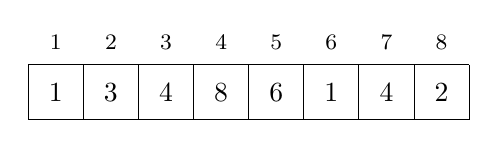
\begin{tikzpicture}[scale=0.7]
\draw (0,0) grid (8,1);

\node at (0.5,0.5) {$1$};
\node at (1.5,0.5) {$3$};
\node at (2.5,0.5) {$4$};
\node at (3.5,0.5) {$8$};
\node at (4.5,0.5) {$6$};
\node at (5.5,0.5) {$1$};
\node at (6.5,0.5) {$4$};
\node at (7.5,0.5) {$2$};

\footnotesize
\node at (0.5,1.4) {$1$};
\node at (1.5,1.4) {$2$};
\node at (2.5,1.4) {$3$};
\node at (3.5,1.4) {$4$};
\node at (4.5,1.4) {$5$};
\node at (5.5,1.4) {$6$};
\node at (6.5,1.4) {$7$};
\node at (7.5,1.4) {$8$};
\end{tikzpicture}
\end{center}


L'arbre binari indexat corresponent és el següent:
\begin{center}
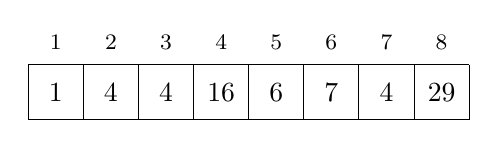
\begin{tikzpicture}[scale=0.7]
\draw (0,0) grid (8,1);

\node at (0.5,0.5) {$1$};
\node at (1.5,0.5) {$4$};
\node at (2.5,0.5) {$4$};
\node at (3.5,0.5) {$16$};
\node at (4.5,0.5) {$6$};
\node at (5.5,0.5) {$7$};
\node at (6.5,0.5) {$4$};
\node at (7.5,0.5) {$29$};

\footnotesize
\node at (0.5,1.4) {$1$};
\node at (1.5,1.4) {$2$};
\node at (2.5,1.4) {$3$};
\node at (3.5,1.4) {$4$};
\node at (4.5,1.4) {$5$};
\node at (5.5,1.4) {$6$};
\node at (6.5,1.4) {$7$};
\node at (7.5,1.4) {$8$};
\end{tikzpicture}
\end{center}


La imatge següent mostra més clarament com cada valor de l'arbre
binari indexat correspon a un interval del vector original:


\begin{center}
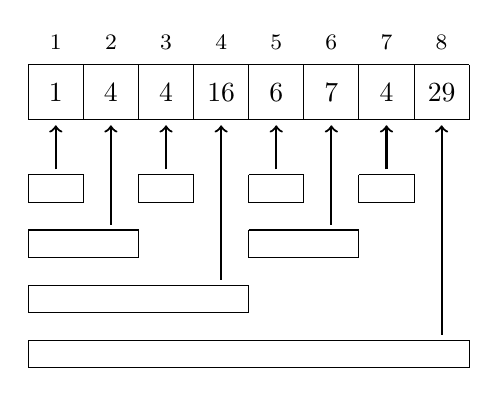
\begin{tikzpicture}[scale=0.7]
\draw (0,0) grid (8,1);

\node at (0.5,0.5) {$1$};
\node at (1.5,0.5) {$4$};
\node at (2.5,0.5) {$4$};
\node at (3.5,0.5) {$16$};
\node at (4.5,0.5) {$6$};
\node at (5.5,0.5) {$7$};
\node at (6.5,0.5) {$4$};
\node at (7.5,0.5) {$29$};

\footnotesize
\node at (0.5,1.4) {$1$};
\node at (1.5,1.4) {$2$};
\node at (2.5,1.4) {$3$};
\node at (3.5,1.4) {$4$};
\node at (4.5,1.4) {$5$};
\node at (5.5,1.4) {$6$};
\node at (6.5,1.4) {$7$};
\node at (7.5,1.4) {$8$};

\draw[->,thick] (0.5,-0.9) -- (0.5,-0.1);
\draw[->,thick] (2.5,-0.9) -- (2.5,-0.1);
\draw[->,thick] (4.5,-0.9) -- (4.5,-0.1);
\draw[->,thick] (6.5,-0.9) -- (6.5,-0.1);
\draw[->,thick] (1.5,-1.9) -- (1.5,-0.1);
\draw[->,thick] (5.5,-1.9) -- (5.5,-0.1);
\draw[->,thick] (3.5,-2.9) -- (3.5,-0.1);
\draw[->,thick] (7.5,-3.9) -- (7.5,-0.1);

\draw (0,-1) -- (1,-1) -- (1,-1.5) -- (0,-1.5) -- (0,-1);
\draw (2,-1) -- (3,-1) -- (3,-1.5) -- (2,-1.5) -- (2,-1);
\draw (4,-1) -- (5,-1) -- (5,-1.5) -- (4,-1.5) -- (4,-1);
\draw (6,-1) -- (7,-1) -- (7,-1.5) -- (6,-1.5) -- (6,-1);
\draw (0,-2) -- (2,-2) -- (2,-2.5) -- (0,-2.5) -- (0,-2);
\draw (4,-2) -- (6,-2) -- (6,-2.5) -- (4,-2.5) -- (4,-2);
\draw (0,-3) -- (4,-3) -- (4,-3.5) -- (0,-3.5) -- (0,-3);
\draw (0,-4) -- (8,-4) -- (8,-4.5) -- (0,-4.5) -- (0,-4);
\end{tikzpicture}
\end{center}


Fent servir un arbre binari indexat, qualsevol valor de $\texttt{sum}_q(1,k)$ es pot
calcular en temps $O(\log n)$, perquè un interval $[1,k]$ sempre es pot dividir en
$O(\log n)$ intervals les sumes dels quals estan emmgatzemades a l'arbre.

Per exemple, l'interval $[1,7]$ consta dels intervals següents:
\begin{center}
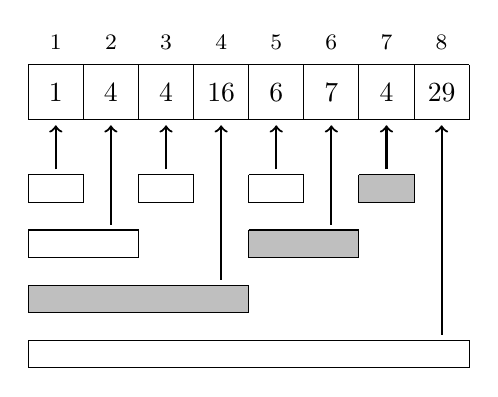
\begin{tikzpicture}[scale=0.7]
\draw (0,0) grid (8,1);

\node at (0.5,0.5) {$1$};
\node at (1.5,0.5) {$4$};
\node at (2.5,0.5) {$4$};
\node at (3.5,0.5) {$16$};
\node at (4.5,0.5) {$6$};
\node at (5.5,0.5) {$7$};
\node at (6.5,0.5) {$4$};
\node at (7.5,0.5) {$29$};

\footnotesize
\node at (0.5,1.4) {$1$};
\node at (1.5,1.4) {$2$};
\node at (2.5,1.4) {$3$};
\node at (3.5,1.4) {$4$};
\node at (4.5,1.4) {$5$};
\node at (5.5,1.4) {$6$};
\node at (6.5,1.4) {$7$};
\node at (7.5,1.4) {$8$};

\draw[->,thick] (0.5,-0.9) -- (0.5,-0.1);
\draw[->,thick] (2.5,-0.9) -- (2.5,-0.1);
\draw[->,thick] (4.5,-0.9) -- (4.5,-0.1);
\draw[->,thick] (6.5,-0.9) -- (6.5,-0.1);
\draw[->,thick] (1.5,-1.9) -- (1.5,-0.1);
\draw[->,thick] (5.5,-1.9) -- (5.5,-0.1);
\draw[->,thick] (3.5,-2.9) -- (3.5,-0.1);
\draw[->,thick] (7.5,-3.9) -- (7.5,-0.1);

\draw (0,-1) -- (1,-1) -- (1,-1.5) -- (0,-1.5) -- (0,-1);
\draw (2,-1) -- (3,-1) -- (3,-1.5) -- (2,-1.5) -- (2,-1);
\draw (4,-1) -- (5,-1) -- (5,-1.5) -- (4,-1.5) -- (4,-1);
\draw[fill=lightgray] (6,-1) -- (7,-1) -- (7,-1.5) -- (6,-1.5) -- (6,-1);
\draw (0,-2) -- (2,-2) -- (2,-2.5) -- (0,-2.5) -- (0,-2);
\draw[fill=lightgray] (4,-2) -- (6,-2) -- (6,-2.5) -- (4,-2.5) -- (4,-2);
\draw[fill=lightgray] (0,-3) -- (4,-3) -- (4,-3.5) -- (0,-3.5) -- (0,-3);
\draw (0,-4) -- (8,-4) -- (8,-4.5) -- (0,-4.5) -- (0,-4);
\end{tikzpicture}
\end{center}
Així, podem calcular la suma corresponent de la següent manera:
\[\texttt{sum}_q(1,7)=\texttt{sum}_q(1,4)+\texttt{sum}_q(5,6)+\texttt{sum}_q(7,7)=16+7+4=27\]


Per calcular el valor de $\texttt{sum}_q(a,b)$ on $a>1$, podem fem servir el mateix
truc que hem fet servir amb els vectors suma de prefixos:
\[ \texttt{sum}_q(a,b) = \texttt{sum}_q(1,b) - \texttt{sum}_q(1,a-1).\]
Com que podem calcular tant $\texttt{sum}_q(1,b)$ com
$\texttt{sum}_q(1,a-1)$ en temps $O(\log n)$, la complexitat total és $O(\log n)$.

Quan actualitzem un valor en el vector original, hem
d'actualitzar diversos valors de l'arbre binari indexat. Per exemple,
si el valor a la posició 3 canvia, les sumes dels intervals següents
canvien:
\begin{center}
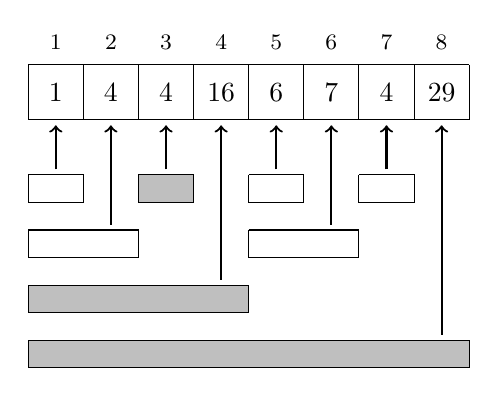
\begin{tikzpicture}[scale=0.7]
\draw (0,0) grid (8,1);

\node at (0.5,0.5) {$1$};
\node at (1.5,0.5) {$4$};
\node at (2.5,0.5) {$4$};
\node at (3.5,0.5) {$16$};
\node at (4.5,0.5) {$6$};
\node at (5.5,0.5) {$7$};
\node at (6.5,0.5) {$4$};
\node at (7.5,0.5) {$29$};

\footnotesize
\node at (0.5,1.4) {$1$};
\node at (1.5,1.4) {$2$};
\node at (2.5,1.4) {$3$};
\node at (3.5,1.4) {$4$};
\node at (4.5,1.4) {$5$};
\node at (5.5,1.4) {$6$};
\node at (6.5,1.4) {$7$};
\node at (7.5,1.4) {$8$};

\draw[->,thick] (0.5,-0.9) -- (0.5,-0.1);
\draw[->,thick] (2.5,-0.9) -- (2.5,-0.1);
\draw[->,thick] (4.5,-0.9) -- (4.5,-0.1);
\draw[->,thick] (6.5,-0.9) -- (6.5,-0.1);
\draw[->,thick] (1.5,-1.9) -- (1.5,-0.1);
\draw[->,thick] (5.5,-1.9) -- (5.5,-0.1);
\draw[->,thick] (3.5,-2.9) -- (3.5,-0.1);
\draw[->,thick] (7.5,-3.9) -- (7.5,-0.1);

\draw (0,-1) -- (1,-1) -- (1,-1.5) -- (0,-1.5) -- (0,-1);
\draw[fill=lightgray] (2,-1) -- (3,-1) -- (3,-1.5) -- (2,-1.5) -- (2,-1);
\draw (4,-1) -- (5,-1) -- (5,-1.5) -- (4,-1.5) -- (4,-1);
\draw (6,-1) -- (7,-1) -- (7,-1.5) -- (6,-1.5) -- (6,-1);
\draw (0,-2) -- (2,-2) -- (2,-2.5) -- (0,-2.5) -- (0,-2);
\draw (4,-2) -- (6,-2) -- (6,-2.5) -- (4,-2.5) -- (4,-2);
\draw[fill=lightgray] (0,-3) -- (4,-3) -- (4,-3.5) -- (0,-3.5) -- (0,-3);
\draw[fill=lightgray] (0,-4) -- (8,-4) -- (8,-4.5) -- (0,-4.5) -- (0,-4);
\end{tikzpicture}
\end{center}


Com que cada element del vector pertany a $O(\log n)$ intervals de
l'arbre binari indexat, n'hi ha prou amb actualitzar $O(\log n)$
valors de l'arbre.

\subsubsection{Implementació}

Les operacions d'un arbre binari indexat es poden implementar de
manera eficient mitjançant operacions de bits. El fet clau és que
podem calcular qualsevol valor de $p(k)$ mitjançant la fórmula
\[p(k) = k \& -k.\]


La funció següent calcula el valor de $\texttt{sum}_q(1,k)$:
\begin{lstlisting}
int sum(int k) {
    int s = 0;
    while (k >= 1) {
        s += tree[k];
        k -= k&-k;
    }
    return s;
}
\end{lstlisting}


La funció següent augmenta en $x$ unitats el valor del vector a la posició $k$
($x$ pot ser positiu o negatiu):
\begin{lstlisting}
void add(int k, int x) {
    while (k <= n) {
        tree[k] += x;
        k += k&-k;
    }
}
\end{lstlisting}


La complexitat temporal d'ambdues funcions és $O(\log n)$, perquè les
funcions accedeixen als $O(\log n)$ valors de l'arbre binari indexat, i
cada moviment a la següent posició triga temps $O(1)$.

\section{Arbre de segments} \label{arbres-segments}

\index{arbre de segments} \index{segment tree}

Un \key{arbre de segments}\footnote{La implementació de baix a dalt
d'aquest capítol correspon a la de \cite{sta06}. Estructures similars
es van fent servir a finals dels 70 per a resoldre problemes
geomètrics \cite{ben80}.} (\emph{segment tree}) és una estructura de
dades que admet dues operacions: processar una consulta d'interval i
actualitzar un valor del vector. Els arbres de segments poden suportar
consultes de suma, consultes de mínim i màxim i moltes altres
consultes perquè ambdues operacions funcionen en $O(\log n)$ temps.

En comparació amb un arbre binari indexat, l'avantatge d'un arbre de
segments és que és una estructura de dades més general. Tot i que els
arbres indexats binaris només admeten consultes de suma\footnote{De
fet, utilitzant \emph{dos} arbres indexats binaris és possible
suportar consultes de mínim \cite{dim15}, però és més complicat
que utilitzar un arbre de segments.}, Els arbres de segments també
admeten altres consultes. D'altra banda, un arbre de segments
requereix més memòria i és una mica més difícil d'implementar.

\subsubsection{Estructura}

Un arbre de segments és un arbre binari on els nodes del nivell inferior de l'arbre
corresponen als elements del vector i els altres nodes contenen la informació
necessària per a processar les consultes d'interval.

En aquesta secció, suposem que la mida del vector és una potència de
dos i utilitzem una indexació basada en zero, perquè resulta més
convenient.  Si la mida del vector no és una potència de dos, sempre
podem afegir-hi elements addicionals.

Primer parlarem dels arbres de segments que admeten consultes de
suma. Com a exemple, considereu el vector següent:
\begin{center}
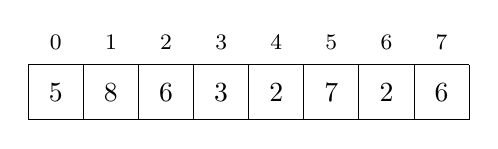
\begin{tikzpicture}[scale=0.7]
\draw (0,0) grid (8,1);

\node at (0.5,0.5) {$5$};
\node at (1.5,0.5) {$8$};
\node at (2.5,0.5) {$6$};
\node at (3.5,0.5) {$3$};
\node at (4.5,0.5) {$2$};
\node at (5.5,0.5) {$7$};
\node at (6.5,0.5) {$2$};
\node at (7.5,0.5) {$6$};

\footnotesize
\node at (0.5,1.4) {$0$};
\node at (1.5,1.4) {$1$};
\node at (2.5,1.4) {$2$};
\node at (3.5,1.4) {$3$};
\node at (4.5,1.4) {$4$};
\node at (5.5,1.4) {$5$};
\node at (6.5,1.4) {$6$};
\node at (7.5,1.4) {$7$};
\end{tikzpicture}
\end{center}
L'arbre de segments corresponent és el següent:
\begin{center}
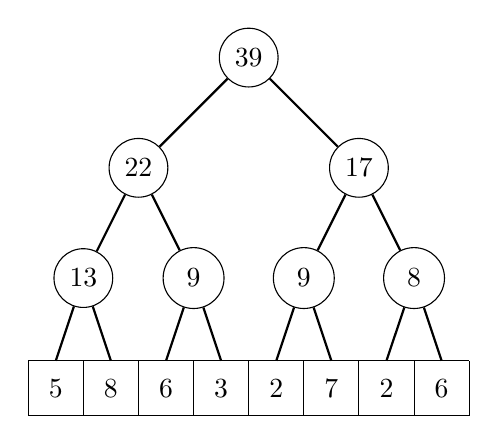
\begin{tikzpicture}[scale=0.7]
\draw (0,0) grid (8,1);

\node[anchor=center] at (0.5, 0.5) {5};
\node[anchor=center] at (1.5, 0.5) {8};
\node[anchor=center] at (2.5, 0.5) {6};
\node[anchor=center] at (3.5, 0.5) {3};
\node[anchor=center] at (4.5, 0.5) {2};
\node[anchor=center] at (5.5, 0.5) {7};
\node[anchor=center] at (6.5, 0.5) {2};
\node[anchor=center] at (7.5, 0.5) {6};

\node[draw, circle] (a) at (1,2.5) {13};
\path[draw,thick,-] (a) -- (0.5,1);
\path[draw,thick,-] (a) -- (1.5,1);
\node[draw, circle,minimum size=22pt] (b) at (3,2.5) {9};
\path[draw,thick,-] (b) -- (2.5,1);
\path[draw,thick,-] (b) -- (3.5,1);
\node[draw, circle,minimum size=22pt] (c) at (5,2.5) {9};
\path[draw,thick,-] (c) -- (4.5,1);
\path[draw,thick,-] (c) -- (5.5,1);
\node[draw, circle,minimum size=22pt] (d) at (7,2.5) {8};
\path[draw,thick,-] (d) -- (6.5,1);
\path[draw,thick,-] (d) -- (7.5,1);

\node[draw, circle] (i) at (2,4.5) {22};
\path[draw,thick,-] (i) -- (a);
\path[draw,thick,-] (i) -- (b);
\node[draw, circle] (j) at (6,4.5) {17};
\path[draw,thick,-] (j) -- (c);
\path[draw,thick,-] (j) -- (d);

\node[draw, circle] (m) at (4,6.5) {39};
\path[draw,thick,-] (m) -- (i);
\path[draw,thick,-] (m) -- (j);
\end{tikzpicture}
\end{center}


Cada node intern de l'arbre es correspon a un interval del vector la
mida del qual és una potència de dos. En l'arbre anterior, el valor de
cada node intern és la suma dels valors corresponents del vector i es
pot calcular com la suma dels valors del fill esquerre i dret.

Resulta que qualsevol rang $[a,b]$ es pot dividir en $O(\log n)$ els valors dels
quals s'emmagatzemen als nodes de l'arbre. Per exemple, considereu l'interval [2,7]:
\begin{center}
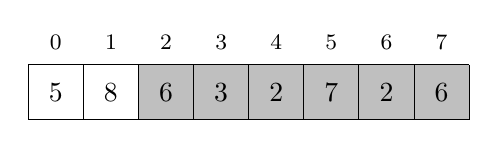
\begin{tikzpicture}[scale=0.7]
\fill[color=gray!50] (2,0) rectangle (8,1);
\draw (0,0) grid (8,1);

\node[anchor=center] at (0.5, 0.5) {5};
\node[anchor=center] at (1.5, 0.5) {8};
\node[anchor=center] at (2.5, 0.5) {6};
\node[anchor=center] at (3.5, 0.5) {3};
\node[anchor=center] at (4.5, 0.5) {2};
\node[anchor=center] at (5.5, 0.5) {7};
\node[anchor=center] at (6.5, 0.5) {2};
\node[anchor=center] at (7.5, 0.5) {6};

\footnotesize
\node at (0.5,1.4) {$0$};
\node at (1.5,1.4) {$1$};
\node at (2.5,1.4) {$2$};
\node at (3.5,1.4) {$3$};
\node at (4.5,1.4) {$4$};
\node at (5.5,1.4) {$5$};
\node at (6.5,1.4) {$6$};
\node at (7.5,1.4) {$7$};
\end{tikzpicture}
\end{center}
Aquí $\texttt{sum}_q(2,7)=6+3+2+7+2+6=26$. En aquest cas, els dos nodes
següents es corresponen amb l'interval:
\begin{center}
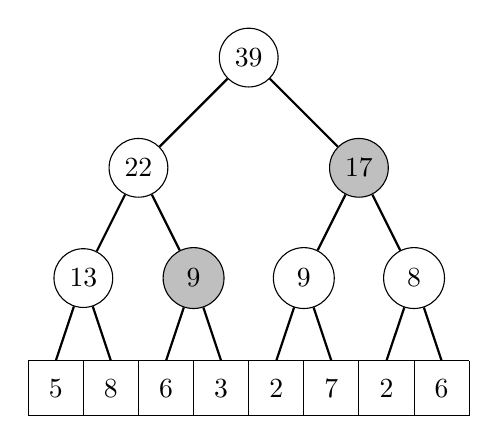
\begin{tikzpicture}[scale=0.7]
\draw (0,0) grid (8,1);

\node[anchor=center] at (0.5, 0.5) {5};
\node[anchor=center] at (1.5, 0.5) {8};
\node[anchor=center] at (2.5, 0.5) {6};
\node[anchor=center] at (3.5, 0.5) {3};
\node[anchor=center] at (4.5, 0.5) {2};
\node[anchor=center] at (5.5, 0.5) {7};
\node[anchor=center] at (6.5, 0.5) {2};
\node[anchor=center] at (7.5, 0.5) {6};

\node[draw, circle] (a) at (1,2.5) {13};
\path[draw,thick,-] (a) -- (0.5,1);
\path[draw,thick,-] (a) -- (1.5,1);
\node[draw, circle,fill=gray!50,minimum size=22pt] (b) at (3,2.5) {9};
\path[draw,thick,-] (b) -- (2.5,1);
\path[draw,thick,-] (b) -- (3.5,1);
\node[draw, circle,minimum size=22pt] (c) at (5,2.5) {9};
\path[draw,thick,-] (c) -- (4.5,1);
\path[draw,thick,-] (c) -- (5.5,1);
\node[draw, circle,minimum size=22pt] (d) at (7,2.5) {8};
\path[draw,thick,-] (d) -- (6.5,1);
\path[draw,thick,-] (d) -- (7.5,1);

\node[draw, circle] (i) at (2,4.5) {22};
\path[draw,thick,-] (i) -- (a);
\path[draw,thick,-] (i) -- (b);
\node[draw, circle,fill=gray!50] (j) at (6,4.5) {17};
\path[draw,thick,-] (j) -- (c);
\path[draw,thick,-] (j) -- (d);

\node[draw, circle] (m) at (4,6.5) {39};
\path[draw,thick,-] (m) -- (i);
\path[draw,thick,-] (m) -- (j);
\end{tikzpicture}
\end{center}
Així, una altra manera de calcular la suma és $9+17=26$.

Quan la suma es calcula fent servir nodes situats el més alt possible a
l'arbre, fan falta com a màxim dos nodes a cada nivell de
l'arbre. Per tant, el nombre total de nodes és $O(\log n)$.

Quan actualitzem un element del vector, hem d'actualitzar tots els
nodes el valor dels quals depèn de l'element actualitzat. Això es pot
fer travessant el camí des de l'element actualitzat fins al node
superior i actualitzant els nodes al llarg del camí.

La imatge següent mostra quins nodes d'arbre canvien si l'element 7
del vector canvia:


\begin{center}
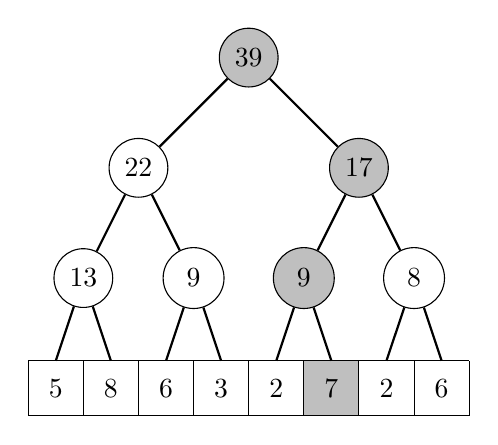
\begin{tikzpicture}[scale=0.7]
\fill[color=gray!50] (5,0) rectangle (6,1);
\draw (0,0) grid (8,1);

\node[anchor=center] at (0.5, 0.5) {5};
\node[anchor=center] at (1.5, 0.5) {8};
\node[anchor=center] at (2.5, 0.5) {6};
\node[anchor=center] at (3.5, 0.5) {3};
\node[anchor=center] at (4.5, 0.5) {2};
\node[anchor=center] at (5.5, 0.5) {7};
\node[anchor=center] at (6.5, 0.5) {2};
\node[anchor=center] at (7.5, 0.5) {6};

\node[draw, circle] (a) at (1,2.5) {13};
\path[draw,thick,-] (a) -- (0.5,1);
\path[draw,thick,-] (a) -- (1.5,1);
\node[draw, circle,minimum size=22pt] (b) at (3,2.5) {9};
\path[draw,thick,-] (b) -- (2.5,1);
\path[draw,thick,-] (b) -- (3.5,1);
\node[draw, circle,minimum size=22pt,fill=gray!50] (c) at (5,2.5) {9};
\path[draw,thick,-] (c) -- (4.5,1);
\path[draw,thick,-] (c) -- (5.5,1);
\node[draw, circle,minimum size=22pt] (d) at (7,2.5) {8};
\path[draw,thick,-] (d) -- (6.5,1);
\path[draw,thick,-] (d) -- (7.5,1);

\node[draw, circle] (i) at (2,4.5) {22};
\path[draw,thick,-] (i) -- (a);
\path[draw,thick,-] (i) -- (b);
\node[draw, circle,fill=gray!50] (j) at (6,4.5) {17};
\path[draw,thick,-] (j) -- (c);
\path[draw,thick,-] (j) -- (d);

\node[draw, circle,fill=gray!50] (m) at (4,6.5) {39};
\path[draw,thick,-] (m) -- (i);
\path[draw,thick,-] (m) -- (j);
\end{tikzpicture}
\end{center}


El camí de baix a dalt sempre consta de $O(\log n)$ nodes, de manera
que cada actualització té aquest cost.

\subsubsection{Implementació}

Emmagatzemem un arbre de segments com un vector de $2n$ elements on
$n$ és la mida potència de dos del vector original. Els nodes de
l'arbre s'emmagatzemen de dalt a baix: $\texttt{tree}[1]$ és el node
superior, $\texttt{tree}[2]$ i $\texttt{tree}[3]$ són els seus fills,
etcètera. Finalment, els valors de $\texttt{tree}[n]$ a
$\texttt{tree}[2n-1]$ corresponen als valors del vector original al
nivell inferior de l'arbre.

Per exemple, l'arbre de segments
\begin{center}
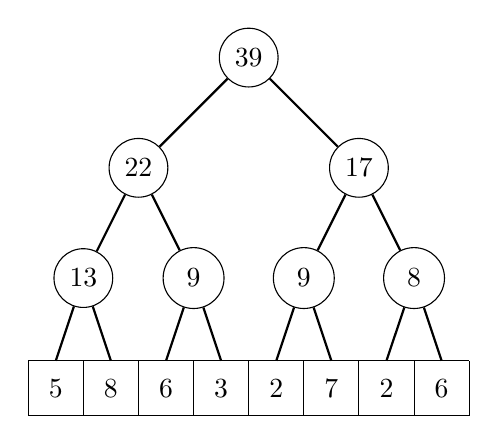
\begin{tikzpicture}[scale=0.7]
\draw (0,0) grid (8,1);

\node[anchor=center] at (0.5, 0.5) {5};
\node[anchor=center] at (1.5, 0.5) {8};
\node[anchor=center] at (2.5, 0.5) {6};
\node[anchor=center] at (3.5, 0.5) {3};
\node[anchor=center] at (4.5, 0.5) {2};
\node[anchor=center] at (5.5, 0.5) {7};
\node[anchor=center] at (6.5, 0.5) {2};
\node[anchor=center] at (7.5, 0.5) {6};

\node[draw, circle] (a) at (1,2.5) {13};
\path[draw,thick,-] (a) -- (0.5,1);
\path[draw,thick,-] (a) -- (1.5,1);
\node[draw, circle,minimum size=22pt] (b) at (3,2.5) {9};
\path[draw,thick,-] (b) -- (2.5,1);
\path[draw,thick,-] (b) -- (3.5,1);
\node[draw, circle,minimum size=22pt] (c) at (5,2.5) {9};
\path[draw,thick,-] (c) -- (4.5,1);
\path[draw,thick,-] (c) -- (5.5,1);
\node[draw, circle,minimum size=22pt] (d) at (7,2.5) {8};
\path[draw,thick,-] (d) -- (6.5,1);
\path[draw,thick,-] (d) -- (7.5,1);

\node[draw, circle] (i) at (2,4.5) {22};
\path[draw,thick,-] (i) -- (a);
\path[draw,thick,-] (i) -- (b);
\node[draw, circle] (j) at (6,4.5) {17};
\path[draw,thick,-] (j) -- (c);
\path[draw,thick,-] (j) -- (d);

\node[draw, circle] (m) at (4,6.5) {39};
\path[draw,thick,-] (m) -- (i);
\path[draw,thick,-] (m) -- (j);
\end{tikzpicture}
\end{center}
s'emmagatzema de la manera següent:
\begin{center}
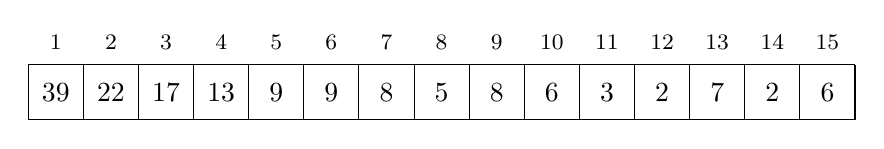
\begin{tikzpicture}[scale=0.7]
\draw (0,0) grid (15,1);

\node at (0.5,0.5) {$39$};
\node at (1.5,0.5) {$22$};
\node at (2.5,0.5) {$17$};
\node at (3.5,0.5) {$13$};
\node at (4.5,0.5) {$9$};
\node at (5.5,0.5) {$9$};
\node at (6.5,0.5) {$8$};
\node at (7.5,0.5) {$5$};
\node at (8.5,0.5) {$8$};
\node at (9.5,0.5) {$6$};
\node at (10.5,0.5) {$3$};
\node at (11.5,0.5) {$2$};
\node at (12.5,0.5) {$7$};
\node at (13.5,0.5) {$2$};
\node at (14.5,0.5) {$6$};

\footnotesize
\node at (0.5,1.4) {$1$};
\node at (1.5,1.4) {$2$};
\node at (2.5,1.4) {$3$};
\node at (3.5,1.4) {$4$};
\node at (4.5,1.4) {$5$};
\node at (5.5,1.4) {$6$};
\node at (6.5,1.4) {$7$};
\node at (7.5,1.4) {$8$};
\node at (8.5,1.4) {$9$};
\node at (9.5,1.4) {$10$};
\node at (10.5,1.4) {$11$};
\node at (11.5,1.4) {$12$};
\node at (12.5,1.4) {$13$};
\node at (13.5,1.4) {$14$};
\node at (14.5,1.4) {$15$};
\end{tikzpicture}
\end{center}
Fent servir aquesta representació, el pare de $\texttt{tree}[k]$ és
$\texttt{tree}[\lfloor k/2 \rfloor]$, i els seus fills són
$\texttt{tree}[2k]$ i $\texttt{tree}[2k+1]$. Tingueu en compte que
això implica que la posició d'un node és parell si és fill esquerre
i imparell si és fill dret.

La funció següent calcula el valor de $\texttt{sum}_q(a,b)$:
\begin{lstlisting}
int sum(int a, int b) {
    a += n; b += n;
    int s = 0;
    while (a <= b) {
        if (a%2 == 1) s += tree[a++];
        if (b%2 == 0) s += tree[b--];
        a /= 2; b /= 2;
    }
    return s;
}
\end{lstlisting}
La funció manté un interval que inicialment és $[a+n,b+n]$. Aleshores, a
cada pas, l'interval es mou al nivell superior en l'arbre, i abans
d'això, els valors dels nodes que no pertanyen a l'interval superior
s'afegeixen a la suma.

La funció següent incrementa en $x$ unitats l'element a la posició $k$ del vector:
\begin{lstlisting}
void add(int k, int x) {
    k += n;
    tree[k] += x;
    for (k /= 2; k >= 1; k /= 2) {
        tree[k] = tree[2*k]+tree[2*k+1];
    }
}
\end{lstlisting}
Primer, la funció actualitza el valor al nivell inferior de
l'arbre. Després d'això, la funció actualitza els valors de tots els
nodes interns de l'arbre, fins que arriba al node superior de l'arbre.

Les dues funcions anteriors funcionen en temps $O(\log n)$, perquè un
arbre de segments de $n$ elements consta de $O(\log n)$ nivells, i les
funcions pugen l'arbre un nivell a cada pas.

\subsubsection{Altres consultes}

Els arbres de segments poden suportar totes les consultes d'interval
on és possible dividir un interval en dues parts, calcular la resposta
per separat per a ambdues parts i després combinar les respostes de
manera eficient. Exemples d'aquestes consultes són el mínim i el
màxim, el màxim comú divisor i les operacions de bits \emph{and},
\emph{or} i \emph{xor}.

Per exemple, l'arbre de segment següent admet consultes de mínim:


\begin{center}
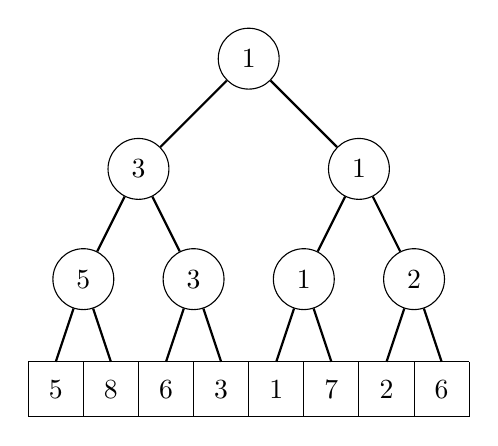
\begin{tikzpicture}[scale=0.7]
\draw (0,0) grid (8,1);

\node[anchor=center] at (0.5, 0.5) {5};
\node[anchor=center] at (1.5, 0.5) {8};
\node[anchor=center] at (2.5, 0.5) {6};
\node[anchor=center] at (3.5, 0.5) {3};
\node[anchor=center] at (4.5, 0.5) {1};
\node[anchor=center] at (5.5, 0.5) {7};
\node[anchor=center] at (6.5, 0.5) {2};
\node[anchor=center] at (7.5, 0.5) {6};

\node[draw, circle,minimum size=22pt] (a) at (1,2.5) {5};
\path[draw,thick,-] (a) -- (0.5,1);
\path[draw,thick,-] (a) -- (1.5,1);
\node[draw, circle,minimum size=22pt] (b) at (3,2.5) {3};
\path[draw,thick,-] (b) -- (2.5,1);
\path[draw,thick,-] (b) -- (3.5,1);
\node[draw, circle,minimum size=22pt] (c) at (5,2.5) {1};
\path[draw,thick,-] (c) -- (4.5,1);
\path[draw,thick,-] (c) -- (5.5,1);
\node[draw, circle,minimum size=22pt] (d) at (7,2.5) {2};
\path[draw,thick,-] (d) -- (6.5,1);
\path[draw,thick,-] (d) -- (7.5,1);

\node[draw, circle,minimum size=22pt] (i) at (2,4.5) {3};
\path[draw,thick,-] (i) -- (a);
\path[draw,thick,-] (i) -- (b);
\node[draw, circle,minimum size=22pt] (j) at (6,4.5) {1};
\path[draw,thick,-] (j) -- (c);
\path[draw,thick,-] (j) -- (d);

\node[draw, circle,minimum size=22pt] (m) at (4,6.5) {1};
\path[draw,thick,-] (m) -- (i);
\path[draw,thick,-] (m) -- (j);
\end{tikzpicture}
\end{center}


En aquest cas, cada node d'arbre conté el valor més petit de
l'interval del vector corresponent. El node superior de l'arbre conté
el valor més petit de tot el vector. Les operacions es poden
implementar com abans, però en comptes de sumes, es calculen mínims.

L'estructura d'arbre de segments també ens permet fer servir la cerca
binària per a localitzar elements del vector. Per exemple, si l'arbre
admet consultes de mínims, podem trobar la posició de l'element més
petit en temps $O(\log n)$.

Per exemple, a l'arbre anterior, es pot trobar l'element amb el valor
mínim 1 travessant un camí cap avall des del node superior:


\begin{center}
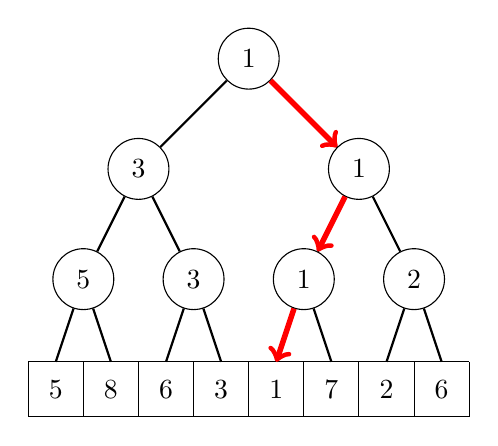
\begin{tikzpicture}[scale=0.7]
\draw (0,0) grid (8,1);

\node[anchor=center] at (0.5, 0.5) {5};
\node[anchor=center] at (1.5, 0.5) {8};
\node[anchor=center] at (2.5, 0.5) {6};
\node[anchor=center] at (3.5, 0.5) {3};
\node[anchor=center] at (4.5, 0.5) {1};
\node[anchor=center] at (5.5, 0.5) {7};
\node[anchor=center] at (6.5, 0.5) {2};
\node[anchor=center] at (7.5, 0.5) {6};

\node[draw, circle,minimum size=22pt] (a) at (1,2.5) {5};
\path[draw,thick,-] (a) -- (0.5,1);
\path[draw,thick,-] (a) -- (1.5,1);
\node[draw, circle,minimum size=22pt] (b) at (3,2.5) {3};
\path[draw,thick,-] (b) -- (2.5,1);
\path[draw,thick,-] (b) -- (3.5,1);
\node[draw, circle,minimum size=22pt] (c) at (5,2.5) {1};
\path[draw,thick,-] (c) -- (4.5,1);
\path[draw,thick,-] (c) -- (5.5,1);
\node[draw, circle,minimum size=22pt] (d) at (7,2.5) {2};
\path[draw,thick,-] (d) -- (6.5,1);
\path[draw,thick,-] (d) -- (7.5,1);

\node[draw, circle,minimum size=22pt] (i) at (2,4.5) {3};
\path[draw,thick,-] (i) -- (a);
\path[draw,thick,-] (i) -- (b);
\node[draw, circle,minimum size=22pt] (j) at (6,4.5) {1};
\path[draw,thick,-] (j) -- (c);
\path[draw,thick,-] (j) -- (d);

\node[draw, circle,minimum size=22pt] (m) at (4,6.5) {1};
\path[draw,thick,-] (m) -- (i);
\path[draw,thick,-] (m) -- (j);

\path[draw=red,thick,->,line width=2pt] (m) -- (j);
\path[draw=red,thick,->,line width=2pt] (j) -- (c);
\path[draw=red,thick,->,line width=2pt] (c) -- (4.5,1);
\end{tikzpicture}
\end{center}


\section{Tècniques addicionals}

\subsubsection{Compressió de l'índex}  \label{compressio-index}

Una limitació de les estructures de dades que es construeixen sobre un
vector és que els elements s'indexen mitjançant nombres enters
consecutius. Les dificultats sorgeixen quan es necessiten índexs
grans. Per exemple, si volem fer servir l'índex $10^9$, el vector
hauria de contenir $10^9$ elements que requeririen massa memòria.

\index{compressió de l'índex}

No obstant això, sovint podem ignorar aquesta limitació fent servir
compressió de l'índex (\key{index compression}), on els índexs
originals es substitueixen per índexs $1,2,3,$, etc. Això es pot fer
si coneixem prèviament tots els índexs necessaris durant l'algorisme.

La idea és substituir cada índex original $x$ per $c(x)$ on $c$ és una
funció que comprimeix els índexs. Necessitem que l'ordre dels índexs
no canviï, de manera que si $a<b$, llavors $c(a)<c(b)$. Això ens
permet realitzar consultes còmodament encara que els índexs estiguin
comprimits.

Per exemple, si els índexs originals són $555$, $10^9$ i $8$, els nous
índexs són:


\[
\begin{array}{lcl}
c(8) & = & 1 \\
c(555) & = & 2 \\
c(10^9) & = & 3 \\
\end{array}
\]


\subsubsection{Actualitzacions d'interval}
\label{actualitzacio-d-intervals}

Fins ara, hem implementat estructures de dades que admeten consultes
d'interval i actualitzacions de valors únics. Considerem ara una
situació oposada, on hauríem d'actualitzar intervals i recuperar
valors únics. Ens centrem en una operació que augmenta tots els
elements d'un interval $[a,b]$ en $x$.

\index{vector de diferències}

Sorprenentment, podem utilitzar les estructures de dades presentades
en aquest capítol també en aquesta situació. Per a fer-ho, construïm
una \key{vector de diferències} els valors del qual indiquen les
diferències entre valors consecutius del vector original. Així, el
vector original és el vector suma de prefixos del vector de
diferències. Per exemple, considereu el vector següent:


\begin{center}
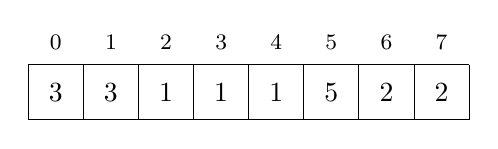
\begin{tikzpicture}[scale=0.7]
\draw (0,0) grid (8,1);

\node at (0.5,0.5) {$3$};
\node at (1.5,0.5) {$3$};
\node at (2.5,0.5) {$1$};
\node at (3.5,0.5) {$1$};
\node at (4.5,0.5) {$1$};
\node at (5.5,0.5) {$5$};
\node at (6.5,0.5) {$2$};
\node at (7.5,0.5) {$2$};


\footnotesize
\node at (0.5,1.4) {$0$};
\node at (1.5,1.4) {$1$};
\node at (2.5,1.4) {$2$};
\node at (3.5,1.4) {$3$};
\node at (4.5,1.4) {$4$};
\node at (5.5,1.4) {$5$};
\node at (6.5,1.4) {$6$};
\node at (7.5,1.4) {$7$};
\end{tikzpicture}
\end{center}


El vector de diferències per al vector anterior és el següent:
\begin{center}
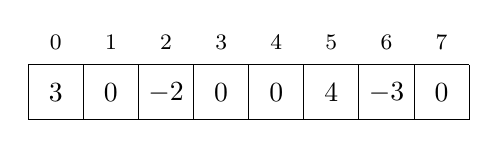
\begin{tikzpicture}[scale=0.7]
\draw (0,0) grid (8,1);

\node at (0.5,0.5) {$3$};
\node at (1.5,0.5) {$0$};
\node at (2.5,0.5) {$-2$};
\node at (3.5,0.5) {$0$};
\node at (4.5,0.5) {$0$};
\node at (5.5,0.5) {$4$};
\node at (6.5,0.5) {$-3$};
\node at (7.5,0.5) {$0$};


\footnotesize
\node at (0.5,1.4) {$0$};
\node at (1.5,1.4) {$1$};
\node at (2.5,1.4) {$2$};
\node at (3.5,1.4) {$3$};
\node at (4.5,1.4) {$4$};
\node at (5.5,1.4) {$5$};
\node at (6.5,1.4) {$6$};
\node at (7.5,1.4) {$7$};
\end{tikzpicture}
\end{center}


Per exemple, el valor 2 a la posició 6 del vector original correspon a la suma $3-2+4-3=2$ al vector de diferències.

L'avantatge del vector de diferències és que podem actualitzar un interval
del vector original canviant només dos elements del vector de
diferències. Per exemple, si volem augmentar en 5 els valors del vector
original entre les posicions 1 i 4, n'hi ha prou amb augmentar en 5
el valor del vector de diferències a la posició 1 i disminuir en 5
el valor a la posició 5. El resultat és el següent:


\begin{center}
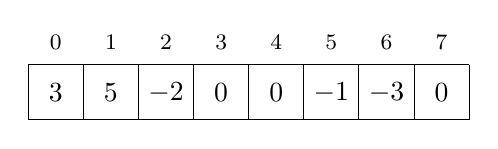
\begin{tikzpicture}[scale=0.7]
\draw (0,0) grid (8,1);

\node at (0.5,0.5) {$3$};
\node at (1.5,0.5) {$5$};
\node at (2.5,0.5) {$-2$};
\node at (3.5,0.5) {$0$};
\node at (4.5,0.5) {$0$};
\node at (5.5,0.5) {$-1$};
\node at (6.5,0.5) {$-3$};
\node at (7.5,0.5) {$0$};

\footnotesize
\node at (0.5,1.4) {$0$};
\node at (1.5,1.4) {$1$};
\node at (2.5,1.4) {$2$};
\node at (3.5,1.4) {$3$};
\node at (4.5,1.4) {$4$};
\node at (5.5,1.4) {$5$};
\node at (6.5,1.4) {$6$};
\node at (7.5,1.4) {$7$};
\end{tikzpicture}
\end{center}


De manera més general, per augmentar en $x$ els valors de l'interval
$[a,b]$, augmentem en $x$ el valor a la posició $a$ i reduïm en $x$ el
valor a la posició $b+1$. Per tant, només cal actualitzar valors
únics i processar consultes de suma, de manera que podem utilitzar un
arbre binari indexat o un arbre de segments.

Un problema més difícil és donar tant suport a les consultes
d'interval com a les actualitzacions d'interval. Al capítol 28 veurem
que fins i tot això és possible.
